\documentclass{standalone}
\makeatletter\AtBeginDocument{\@buildstepset{1,2,3,4}}\makeatother
\usepackage{tikz}
\usetikzlibrary{intersections, calc}
\usepackage{hsbcommon}
\begin{document}
    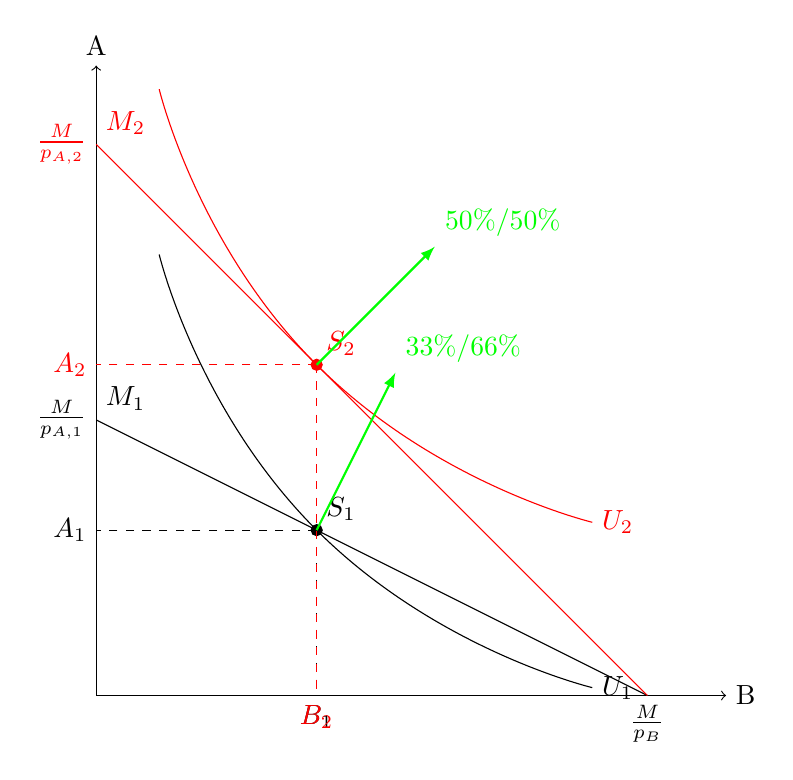
\begin{tikzpicture}
        \draw[->] (0,0) node[below] {\phantom{$X_i$}} -- (8,0) node[right]  {B};
        \draw[->] (0,0) node[left] {\phantom{$Y_mi$}} -- (0,8) node[above]  {A};

        %% Step 1: first budget line (M_1) + indifference curve U_1
        \ifstep{1}{
            \begin{scope}[color=black]
                \coordinate (A1) at (0,3.5);
                \coordinate (B1) at (7,0);
                \node[above right] at (A1) {$M_1$};
                \node[left]        at (A1) {$\frac{M}{p_{A,1}}$};
                \node[below]       at (B1) {$\frac{M}{p_B}$};
                \draw [name path=budgetgerade1] plot [smooth] coordinates {(A1)(B1)};
                \coordinate (S1) at ($(A1)!0.4!(B1)$);
                \node[above right] at (S1) {$S_1$};
                \draw [dashed] (S1) -- (S1 |-,0) node [below] {$B_1$};
                \draw [dashed] (S1) -- (0,|- S1)  node [left]  {$A_1$};
                \filldraw (S1) circle (2pt);
                \coordinate (P1) at ([shift=({-2cm,3.5cm})]S1);
                \coordinate (Q1) at ([shift=({3.5cm,-2cm})]S1);
                \node[right] at (Q1) {$U_1$};
                \draw [name path=indiff1] plot [smooth, tension=1] coordinates {(P1)(S1)(Q1)};
            \end{scope}
        }

        %% Always visible: second budget line (M_2) + indifference curve U_2
        \begin{scope}[color=red]
            \coordinate (A2) at (0,7);
            \coordinate (B2) at (7,0);
            \node[above right] at (A2) {$M_2$};
            \node[left]        at (A2) {$\frac{M}{p_{A,2}}$};
            \draw [name path=budgetgerade2] plot [smooth] coordinates {(A2)(B2)};
            \coordinate (S2) at ($(A2)!0.4!(B2)$);
            \node[above right] at (S2) {$S_2$};
            \draw [dashed] (S2) -- (S2 |-,0) node [below] {$B_2$};
            \draw [dashed] (S2) -- (0,|- S2)  node [left]  {$A_2$};
            \filldraw (S2) circle (2pt);
            \coordinate (P2) at ([shift=({-2cm,3.5cm})]S2);
            \coordinate (Q2) at ([shift=({3.5cm,-2cm})]S2);
            \node[right] at (Q2) {$U_2$};
            \draw [name path=indiff2] plot [smooth, tension=1] coordinates {(P2)(S2)(Q2)};
        \end{scope}

        %% Step 2: arrows showing budget shares
        \ifstep{2}{
            \begin{scope}[color=green]
                \draw[thick,->,>=latex] (S1) -- ([shift=({1cm,2cm})]S1)   node[above right] {33\%/66\%};
                \draw[thick,->,>=latex] (S2) -- ([shift=({1.5cm,1.5cm})]S2) node[above right] {50\%/50\%};
            \end{scope}
        }

    \end{tikzpicture}
\end{document}
